\documentclass{beamer}
% \usepackage{xcolor}
\usepackage{lineno}
\usepackage{minted}
% \usemintedstyle{native}
\usemintedstyle{friendly}
\graphicspath{ {images/} }
\usetheme{boxes}
\setbeamertemplate{blocks}[rounded][shadow=true]

\newenvironment{codeblock}[1]{%
  \setbeamercolor{block body}{bg=white,fg=black}
  \setbeamercolor{block title}{bg=gray,fg=white}
  \begin{block}{#1}}{\end{block}}

\newcommand{\code}[3][]{
  \begin{codeblock}{#2}
  \inputminted[fontsize=\scriptsize,#1]{python}{#3}
  \end{codeblock}
}
\title{Matplotlib custom tools universe}
\subtitle{https://github.com/fariza/pycon2017}
\author{Optical specialist @ Matrox}
\date{\today}

\begin{document}
\begin{frame}
  \titlepage
\end{frame}

\begin{frame}
  \frametitle{Who is this for?}
  \begin{itemize}
    \item Do you play with a lot of data?
    \item Do you plot?
    \item Do you plot a lot of data?
    \item Do you want to get your hands dirty?
    \item You didn't have anything better to do?
  \end{itemize}
\end{frame}

\begin{frame}
\frametitle{The gui}
\begin{columns}
\begin{column}{0.5\textwidth}
  \begin{itemize}
      \item Key-only tools
      \begin{itemize}
        \item Grid
        \item log
        \item ...
      \end{itemize}
      \item Toolbar buttons
      \begin{itemize}
        \item Home
        \item save
        \item ...
      \end{itemize}
  \end{itemize}
\end{column}
\begin{column}{0.5\textwidth}
  \begin{figure}
  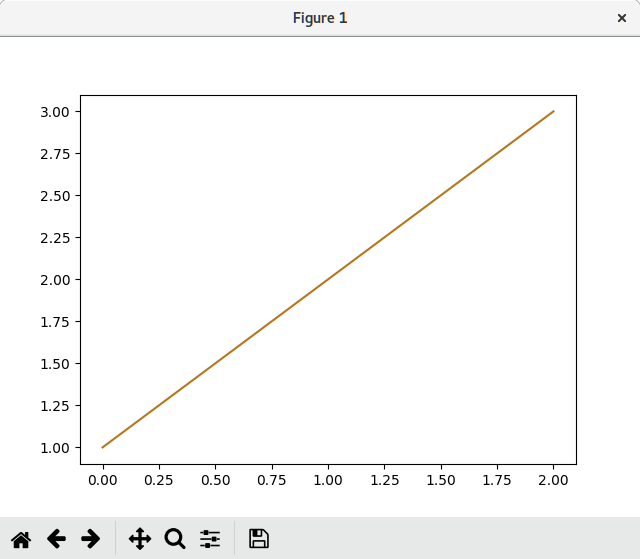
\includegraphics[width=150px]{gui}
  \end{figure}
\end{column}
\end{columns}
\end{frame}

\begin{frame}{Today}
  \begin{block}{Key press events}
      \begin{itemize}
        \item<1-> Single function (Huge, ugly)
        \mint{python} |def key_press_handler(event, canvas, toolbar=None)|
        \item<2-> Some events are transmited to the toolbar
        \item<3-> If no toolbar, then some events are not available
        \item<4-> Some events are handled in place, without possibility for
        for the Toolbar to add a "button"
        \item<5->No easy way to add new key-event handlers
        \item<6->No way to know the associated keys
      \end{itemize}
  \end{block}
\end{frame}

\begin{frame}{Today}
  \begin{block}{Toolbar}
      \begin{itemize}
        \item<1->Base class defines most of the handling
        \item<2->Backend specific code
        \item<3->Gui and process is done in the same place
        \item<4->No "easy" way to call methods inside the toolbar
        \item<5->No way to add new tools without writing a new backend
      \end{itemize}
  \end{block}
\end{frame}

\begin{frame}{New age}
  \begin{block}{Where to find things}
  \begin{figure}
  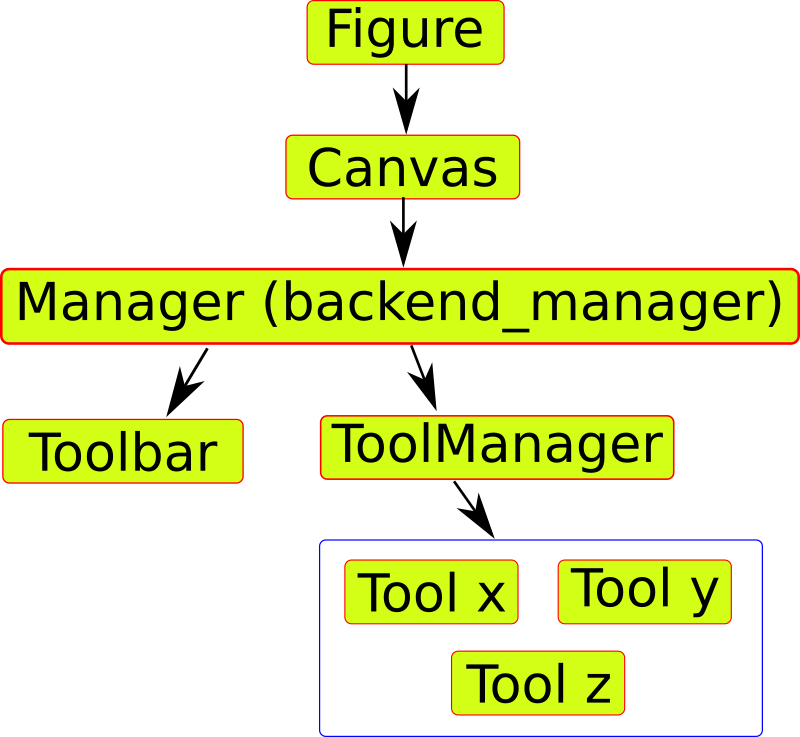
\includegraphics[width=200px]{mpl_classes}
  \end{figure}
\end{block}
\end{frame}


\begin{frame}{New age}
  \begin{block}{ToolManager}
      \begin{itemize}
        \item<1->Add/remove/modify tools dynamically
        \item<2->Does not have any gui related code
        \item<3->Keep track of associated keys
        \item<4->Manage tool radio groups
      \end{itemize}
  \end{block}
\end{frame}

\begin{frame}{New age}
  \begin{block}{Tools}
      \begin{itemize}
        \item<1->Two kind of tools:
        \begin{itemize}
          \item<2->Basic tool
          \item<3->Toggle tool
       \end{itemize}
      \end{itemize}
  \end{block}
\end{frame}

\begin{frame}{New age}
  \begin{block}{Toolbar}
      \begin{itemize}
        \item<1->Has no logic related to tools
        \item<2->Two important methods: addtool, removetool
        \item<3->Hooks to tool-events to change button state if a tool is
        triggered by any way other than "click"
        \item<4->Simple backend creation
      \end{itemize}
  \end{block}
\end{frame}

\begin{frame}{Does it work?}
  \code{Let's check}{code/1-work.py}
\end{frame}

\begin{frame}{Play with buttons}
  \only<1->{\code[lastline=8,firstline=8]{Remove one button}{code/2-clutter.py}}
  \only<2->{\code[lastline=9,firstline=9]{Duplicate a button}{code/2-clutter.py}}
  \only<3->{\code[lastline=10,firstline=10]{Completely remove one button}{code/2-clutter.py}}
\end{frame}

\begin{frame}{Simple tool}
  \only<1->{\code[lastline=13,firstline=5]{Extra-Simple tool}{code/3-simple.py}}
  \only<2->{\code[lastline=17,firstline=17]{Add the tool to toolmanager}{code/3-simple.py}}
  \only<3->{\code[lastline=18,firstline=18]{Add to the toolbar}{code/3-simple.py}}
\end{frame}

\begin{frame}{Toggle tool}
  \code[lastline=25,firstline=5]{Toggle legend}{code/4-legend.py}
\end{frame}

\begin{frame}{Toggle tool}
  \only<1->{\code[lastline=29,firstline=29]{Add a legend}{code/4-legend.py}}
  \only<2->{\code[lastline=31,firstline=30]{Add the tool}{code/4-legend.py}}
\end{frame}


\end{document}
